% Self-contained technical manuscript. Original vector diagrams; no images
% from the source repository are reproduced here.
% Reproducibility snapshot: CambrianMinds/martian-cylinder, master,
% 90fbf8f89ac2634a9dbd2b27f81fc80d68b9943c (2026-11-11).
\documentclass[11pt,letterpaper]{article}
\usepackage[margin=0.92in,headheight=23pt,footskip=30pt]{geometry}
\usepackage[T1]{fontenc}
\usepackage[utf8]{inputenc}
\usepackage{newtxtext,newtxmath}
\usepackage[final]{microtype}
\usepackage{amsmath,mathtools,bm}
\usepackage{booktabs,tabularx,threeparttable,array,multirow}
\usepackage{siunitx}
\usepackage{xcolor}
\usepackage{tikz}
\usetikzlibrary{arrows.meta,calc,patterns,decorations.pathreplacing}
\usepackage{pgfplots}
\pgfplotsset{compat=1.18}
\usepackage{graphicx}
\usepackage{caption,subcaption}
\usepackage{fancyhdr}
\usepackage{titlesec}
\usepackage{enumitem}
\usepackage{hyperref}
\usepackage{cleveref}
\usepackage{listings}
\usepackage{url}
\usepackage{float}
\usepackage{longtable}
\usepackage{needspace}
\usepackage{setspace}
\definecolor{ink}{HTML}{202934}
\definecolor{slate}{HTML}{495B68}
\definecolor{accent}{HTML}{287D84}
\definecolor{pale}{HTML}{E8F0F0}
\definecolor{fine}{HTML}{C9D3D7}
\definecolor{warm}{HTML}{6A5A45}
\hypersetup{colorlinks=true,linkcolor=accent,citecolor=accent,urlcolor=accent,pdftitle={Subpixel Geometric Reconstruction of a Cylindrical Candidate in Curiosity Mastcam-100 Imagery},pdfauthor={Justin Bogner}}
\titleformat{\section}{\color{ink}\large\bfseries}{\thesection.}{0.65em}{}
\titleformat{\subsection}{\color{ink}\normalsize\bfseries}{\thesubsection}{0.65em}{}
\titleformat{\subsubsection}{\color{slate}\normalsize\itshape}{\thesubsubsection}{0.65em}{}
\titlespacing*{\section}{0pt}{20pt}{8pt}
\titlespacing*{\subsection}{0pt}{13pt}{5pt}
\setlength{\parindent}{1.2em}
\setlength{\parskip}{2.5pt}
\setlength{\columnsep}{19pt}
\emergencystretch=2em
\linespread{1.075}
\captionsetup{font=small,labelfont={bf,color=ink},textfont={color=slate},skip=5pt}
\renewcommand\arraystretch{1.15}
\pagestyle{fancy}
\fancyhf{}
\fancyhead[L]{\footnotesize\textsc{Sol 3556 | Mastcam-100}}
\fancyhead[R]{\footnotesize\textsc{Geometric reconstruction}}
\fancyfoot[L]{\footnotesize Bogner \quad | \quad 11 November 2026}
\fancyfoot[R]{\footnotesize\thepage}
\renewcommand{\headrulewidth}{0.4pt}
\renewcommand{\headrule}{\hbox to\headwidth{\color{fine}\leaders\hrule height \headrulewidth\hfill}}
\newcommand{\rms}{\operatorname{RMS}}
\newcommand{\aicc}{\mathrm{AIC}_{\!c}}
\newcommand{\dif}{\mathop{}\!\mathrm{d}}
\newcommand{\px}{\,\mathrm{px}}
\newcommand{\DOF}{\mathrm{DOF}}
\newcommand{\sourcepath}[1]{\nolinkurl{#1}}
\newcommand{\mat}[1]{\mathbf{#1}}
\newcommand{\repo}{\href{https://github.com/CambrianMinds/martian-cylinder}{CambrianMinds/martian-cylinder}}
\newcommand{\pdsid}{\texttt{3556MR1025170721700585C00}}
\lstdefinestyle{code}{basicstyle=\ttfamily\footnotesize,frame=single,rulecolor=\color{fine},backgroundcolor=\color{pale!45},columns=fullflexible,breaklines=true,showstringspaces=false,aboveskip=9pt,belowskip=9pt}
\lstset{style=code}

\begin{document}
\thispagestyle{empty}
\vspace*{-0.24in}
\noindent{\color{accent}\rule{\linewidth}{2.2pt}}\par\vspace{13pt}
{\footnotesize\sffamily\bfseries\color{accent} QUANTITATIVE PLANETARY IMAGE ANALYSIS \quad / \quad RESEARCH ARTICLE}\\[12pt]
{\fontsize{22}{26}\selectfont\bfseries\color{ink} Subpixel Geometric Reconstruction of a Cylindrical Candidate in Curiosity Mastcam-100 Imagery}\\[8pt]
{\large\color{slate} A quantitative analysis of two terminal curves, exterior tangency, partial burial, and competing physical models}\\[17pt]
{\large Justin Bogner}\\[3pt]
{\small\color{slate} Cambrian Minds Media \quad | \quad 11 November 2026}\\[9pt]
{\footnotesize\color{slate} Data and scripts: \repo}\\[2pt]
{\footnotesize\color{slate} Curiosity Sol 3556 \quad / \quad \pdsid}\\[8pt]
\par\noindent{\color{fine}\rule{\linewidth}{0.5pt}}\par

\begin{abstract}
\noindent A centimeter-scale object in Curiosity Mastcam-100 imagery acquired on sol 3556 exhibits two separated curved terminations and a straight upper exterior boundary. We characterize these features using NASA Planetary Data System radiometric products, calibrated CAHVOR/CAHV camera geometry, physically directed subpixel edge localization, orthogonal-distance regression, and coupled geometric models. The analysis identifies 35 near-rim, 24 exposed far-termination, and 26 upper-boundary stations. A freely fitted near-rim ellipse achieves $0.164\px$ orthogonal RMS; a translated copy with identical section size, shape, and orientation matches the far arc at $0.186\px$ RMS. A six-parameter projected right-circular-cylinder model jointly constraining the two terminations, collinear centers, and upper exterior tangency fits all 85 selected observations at $0.3788\px$ total RMS. An eight-parameter coupled tapered model achieves $0.2549\px$, demonstrating a distinct, more flexible image-plane solution. The target's upper edge is four to eight times straighter, by line-fit RMS, than three selected neighboring rock boundaries. Together, the measurements provide reproducible quantitative evidence for cylindrical image-plane morphology, substantially constraining physical explanations. Composition, provenance, and a unique three-dimensional shape remain outside what this single camera view directly measures.
\end{abstract}
\vspace{2pt}
\noindent{\small\textbf{Keywords:} Mars; Gale crater; Curiosity; Mastcam-100; cylinder; subpixel metrology; orthogonal regression; image geometry; occlusion; concretion; technosignature assessment.}\par
\vspace{7pt}
\noindent{\color{fine}\rule{\linewidth}{0.5pt}}\par

\section{Introduction}
\label{sec:intro}

A photograph can establish the projected geometry of an object even when its composition, depth, and origin remain unknown. For the Curiosity Mastcam-100 observation considered here, the central question is unusually specific: can the distinct curved boundary at the foreground end, the exposed curvature at the far end, and the upper longitudinal boundary be represented by one common cylindrical geometry? A secondary question is which physical formation histories can plausibly account for that conjunction.

The target occurs in the image identified by \pdsid, acquired on sol 3556 (7 August 2022). The Mastcam-100 instrument is a fixed-focal-length, narrow-field camera with an instantaneous field of view near \(74\,\mu\mathrm{rad}\) per image pixel, making subpixel analysis appropriate for centimeter-scale objects at several meters' range \cite{malin2017,bell2017}. The target is not a full, free-standing object on a uniform background: its lower outline merges with the regolith, and a dark region adjacent to the near end contains a cast-shadow contribution. Consequently, not every visible intensity transition belongs to the solid's perimeter.

We define material boundaries independently of their suitability for any candidate shape. The upper edge is selected at the bright-body/dark-regolith interface; the lower visible contact is classified as possible foreground soil occlusion rather than automatically being treated as a second silhouette generator. Both terminal curves are registered with explicit parameter constraints. The measured feature families are then tested jointly against constant-section and tapered geometries. The complete image data and executable analyses are archived in the research repository \cite{bogner2026repo}.

This paper reports the resulting measurements, model performance, uncertainty structure, and comparison of candidate formation mechanisms. Observed pixel features, geometric constraints, and interpretations of physical origin are treated as separate levels of inference.

\section{Observational Material and Provenance}
\label{sec:data}

\subsection{Instrument products and pixel conventions}

The primary inputs are NASA PDS3 Reduced Data Record products from the right Mastcam, with product stem \pdsid\ and dataset designation \texttt{MSL-M-MASTCAM-4-RDR-IMG-V1.0}. The investigation operates on zero-based image coordinates \((x,y)\), with \(x\) increasing rightward and \(y\) increasing downward. For the principal radiometric product, an image coordinate refers to the array location in the PDS subframe, not the full detector's absolute position.

\begin{table}[ht]
\centering\small
\caption{Image products and their analytic roles. Dimensions are ordered as image lines \(\times\) samples \(\times\) bands.}
\label{tab:products}
\begin{tabularx}{\linewidth}{@{}l l l X@{}}
\toprule
\textbf{Suffix} & \textbf{Array shape} & \textbf{Encoding} & \textbf{Use in analysis} \\
\midrule
\texttt{DRXX} & \(1184\times1328\times3\) & big-endian 16-bit & Primary radiometric pixel measurements; native CAHVOR geometry \\
\texttt{DRLX} & \(1180\times1323\times3\) & big-endian 16-bit & Independently sampled linearized CAHV geometry \\
\texttt{DRCX} & \(1184\times1328\times3\) & 8-bit & Tonal-display and localization reference \\
\texttt{DRCL} & \(1180\times1323\times3\) & 8-bit & Linearized display and visual comparison \\
\bottomrule
\end{tabularx}
\end{table}

The image metadata give an acquisition time of 2022-08-07 20:58:23.349 UTC, local true solar time 12:10:25, a \(14.2\,\mathrm{ms}\) exposure, and clear-filter Mastcam-right acquisition. The principal data were transmitted with predictive lossless Bayer Huffman compression. Their geometric features therefore are not attributable to JPEG block boundaries. Demosaicing, optical blur, radiometric scaling, and companding nevertheless influence local edge localization and are addressed through multi-band and estimator-sensitivity comparisons.

The per-band radiometric conversion implemented in the repository is
\begin{equation}
I_b(x,y)=o_b+q_b\,\mathrm{DN}_b(x,y),\quad
(q_R,q_G,q_B)=(1.201,1.112,1.037)\times10^{-4},
\label{eq:radiance}
\end{equation}
with \(o_b=0\) in the processed products and radiance in \(\mathrm{W\,m^{-2}\,sr^{-1}\,nm^{-1}}\). The mean of the three band radiances defines the primary scalar field \(I(x,y)\); separate-channel fits provide a check on color interpolation effects.

\subsection{Four distinguishable visual regions}
\label{sec:regions}

The segmentation distinguishes (i) the sunlit longitudinal surface, (ii) its upper background-facing edge, (iii) the foreground curved termination separating illuminated material from the dark recess, and (iv) the lower-right dark patch, whose distal boundary partly follows cast shadow on soil rather than the object's cross-section. The far upper-left termination has its own observable material/background boundary, while its lower part is obscured by regolith.

This classification is causally important. An elliptical fit to a shadow boundary measures illumination geometry and ground topography, not necessarily the perimeter of the object that cast the shadow. Likewise, a line running through the brightest surface is not necessarily the outer silhouette, even if its projected slope is nearly constant.

The analysis reports a regolith-noise estimate \(\sigma_I=7.782\times10^{-3}\) in its radiometric units, a sunlit-object mean near \(9.848\times10^{-2}\), and a dark-core mean near \(1.358\times10^{-2}\), with an edge signal-to-noise estimate of 10.91 for its selected contrast definition. These measurements characterize signal separation without assuming anything about the object's material.

\section{Camera Geometry, Illumination, and Scale}
\label{sec:camera}

\subsection{CAHV and CAHVOR projection}

Let \(\mat C\) be the camera center, \(\mat A\) its optical axis, and \(\mat H,\mat V\) the horizontal and vertical projection vectors. In the linear CAHV model, a three-dimensional point \(\mat P\) projects to
\begin{equation}
 x=\frac{(\mat P-\mat C)\cdot\mat H}{(\mat P-\mat C)\cdot\mat A},\qquad
 y=\frac{(\mat P-\mat C)\cdot\mat V}{(\mat P-\mat C)\cdot\mat A}.
 \label{eq:cahv}
\end{equation}
The corresponding nonlinear CAHVOR model applies radial corrections about distortion axis \(\mat O\):
\begin{align}
\mat p&=\mat P-\mat C, & \omega&=\mat p\cdot\mat O, \\
\bm\lambda&=\frac{\mat p}{\omega}-\mat O, & \tau&=\bm\lambda\cdot\bm\lambda,\\
\mu&=R_0+R_1\tau+R_2\tau^2, &
\mat p'&=\mat p+\mu(\mat p-\omega\mat O).
\end{align}
The corrected vector \(\mat p'\) replaces \(\mat p\) in \cref{eq:cahv}. The script also inverts image coordinates to viewing rays and transforms rover-navigation vectors to the local site reference frame. The independently derived linearized camera azimuth and elevation agree with the recorded pointing values of \(227.7412^\circ\) and \(-22.0047^\circ\), respectively.

At the target location near \((1061,980)\), the singular values of the local angular-to-image Jacobian are \(13{,}498.24\) and \(13{,}418.43\,\mathrm{px\,rad^{-1}}\). Accordingly,
\begin{equation}
 f_{\mathrm{local}}=13{,}458.28\,\mathrm{px\,rad^{-1}},\quad
 \mathrm{IFOV}=74.304\,\mu\mathrm{rad\,px^{-1}},\quad
 \epsilon_{\mathrm{anisotropy}}=0.595\%.
\end{equation}
The small local anisotropy means that a major departure from circularity cannot reasonably be attributed to the lens at this image location.

\subsection{Range-sensitive physical dimensions}

Without an overlapping target stereo solution, angular and pixel-based measurements are better constrained than dimensional measurements in millimeters. Using the metadata's best focus distance \(D_f=3.957\,\mathrm{m}\) as a working range gives a local sampling scale
\begin{equation}
 \ell_{\mathrm{px}}(D)\approx D\,(74.304\times10^{-6})
 = 0.2940\left(\frac{D}{3.957\,\mathrm m}\right)\mathrm{mm\,px^{-1}}.
 \label{eq:scale}
\end{equation}
Within the recorded focus search bracket \(3.6\)--\(4.4\,\mathrm m\), this scale spans approximately \(0.2675\)--\(0.3269\,\mathrm{mm\,px^{-1}}\). A projected strict-model diameter of \(2a\approx39.99\px\) therefore corresponds to \(11.76\,\mathrm{mm}\) at the focus-distance scenario. This is an illustrative physical conversion, not a stereo-derived object range; the true three-dimensional axis length requires an additional orientation estimate.

\subsection{Solar geometry and cast-shadow direction}

PDS metadata give a local solar azimuth of \(186.8169^\circ\) and elevation of \(69.8224^\circ\). Projection through the camera model gives a solar image-plane direction near \(-116.571^\circ\) and a corresponding shadow direction near \(+63.429^\circ\). This direction is consistent with the extensive lower-right dark region. Modeling the shadow as an optical projection onto an underlying soil surface is essential for avoiding an incorrect full-outline fit: the shadow's distal edge need not be concentric with the exposed curved material boundary.

In a simple receiving-plane formulation, let the shadow-casting rim point be \(\mat P\), the unit Sun-direction vector be \(\hat{\mat s}\), and the soil plane satisfy \(\hat{\mat n}_g\cdot(\mat X-\mat P_0)=0\). The physical shadow intersection is
\begin{equation}
 \mat X_{\rm shadow}=\mat P-\lambda\hat{\mat s},\qquad
 \lambda=\frac{\hat{\mat n}_g\cdot(\mat P-\mat P_0)}{\hat{\mat n}_g\cdot\hat{\mat s}},
 \label{eq:shadow}
\end{equation}
when \(\lambda>0\). Camera projection of the resulting point gives the expected image location of the cast shadow. The receiving-plane orientation is a modeled scene property, not an independently measured surface normal. The construction nevertheless explains why the terminal material curve and the lower distal shadow boundary need not be pieces of the same conic.


\section{Subpixel Measurement of Physical Boundaries}
\label{sec:edges}

\subsection{Normal-profile extraction}

For a line segment with unit tangent \(\hat{\mat t}=(t_x,t_y)\), define its directed normal \(\hat{\mat n}=(-t_y,t_x)\). Intensity is sampled on rays
\begin{equation}
 \mat x_i(s)=\mat x_{i,0}+s\hat{\mat n},\qquad
 g_i(s)=I\bigl(\mat x_i(s)\bigr),
\end{equation}
with bilinear interpolation on the radiometric image. After mild Gaussian smoothing, the derivative \(g_i'(s)\) is searched for a contrast extremum of the \emph{physically expected sign}. A local three-sample parabola refines the position; the surrounding unsmoothed profile is also fitted to an error-function transition,
\begin{equation}
 g(s)=I_-+\frac{I_+-I_-}{2}
 \left[1+\operatorname{erf}\left(\frac{s-s_0}{\sqrt 2\,\sigma_{\mathrm{PSF}}}\right)\right],
 \label{eq:erf}
\end{equation}
where \(s_0\) is the transition coordinate, \(\sigma_{\mathrm{PSF}}\) a profile-width parameter, and \(I_\pm\) the fitted asymptotic intensities.

For the upper edge, the selected normal runs from darker background into brighter illuminated object. Its appropriate gradient search polarity is \(+1\). For the lower edge it runs from brighter object into darker soil, requiring \(-1\). The implementation records the sign-adjusted intensity difference across each selected station and checks that the transition follows the expected material boundary.

\subsection{Exterior-boundary validation}
\label{sec:exterior}

The upper boundary is defined by the large, spatially coherent radiometric transition from background regolith into the illuminated body. At each of 26 stations, the extractor records transition contrast, gradient direction, fitted transition position, and fit uncertainty. All 26 stations satisfy the expected polarity diagnostic. Their best-fit line is at $28.895^\circ$, with $0.2422\px$ orthogonal RMS over approximately $36.4\px$ of the visible exterior. The edge-coordinate arrays and diagnostic fields are retained in \sourcepath{step3_features.json}. This feature definition is independent of the subsequent cylinder or tapered-model fits.

\subsection{Near rim: separation from the adjacent pebble}

The near curved termination is sampled at five-degree radial intervals. Of 36 near-rim stations, precisely one at \(\theta=-45^\circ\) lies across a narrow shadow gap on the adjacent upper-right pebble. Its extracted position is approximately \((1083.34,969.16)\), radius \(22.40\px\), compared with neighboring radii of \(19.86\) and \(20.34\px\). The near-rim dataset therefore comprises the 35 stations that lie on the continuous observed termination, with the neighboring pebble excluded by spatial and contrast classification.

\subsection{Far termination: separating cap, soil, and longitudinal transition}

The rear region is sampled from an interior seed at \((1035.5,951.2)\), with radial angles spanning \(-210^\circ\) to \(-35^\circ\). The extractor selects the first outward crossing of a radiometric threshold \(I_{\mathrm{iso}}=0.0860\) before fitting the local transition. The crucial physical partition is between the buried lower-left contact (indices \(0\)--\(7\)), the exposed rear cap (indices \(8\)--\(31\)), and the upper longitudinal transition (indices \(32\)--\(35\)). Only the 24 middle samples are treated as the terminating curve. This prevents a soil-occlusion line from masquerading as a noncircular end.

\section{Curve Fitting and Geometric Models}
\label{sec:models}

\subsection{Orthogonal-distance estimation}

Straightness is estimated using total least squares. For observations \(\{\mat x_i\}\), the eigenvector of the smaller eigenvalue of the 2D sample covariance gives the line normal \(\hat{\mat n}\). Its signed orthogonal residual is
\begin{equation}
 e_i=\hat{\mat n}\cdot(\mat x_i-\bar{\mat x}),\qquad
 \rms_{\perp}=\sqrt{N^{-1}\sum_i e_i^2}.
\end{equation}

For the end curves, an image-plane ellipse centered on \(\mat c\) is parameterized in coordinates aligned with a trial body axis \(\theta\):
\begin{align}
 \hat{\mat u}&=(\cos\theta,\sin\theta), &
 \hat{\mat v}&=(-\sin\theta,\cos\theta),\\
 \mat x(\psi)&=\mat c+b\cos\psi\,\hat{\mat u}
 +a\sin\psi\,\hat{\mat v},
 \label{eq:ellipse}
\end{align}
where \(a\) is the transverse semi-major axis and \(b\) the longitudinally aligned semi-minor axis. A point's residual is its minimum Euclidean distance to the curve, rather than a raw algebraic-conic residual. Newton refinement provides the closest curve point within each nonlinear least-squares evaluation.

\subsection{Uncoupled reference fits}

The 35 clean near-rim observations produce a freely oriented ellipse with \(a=19.7170\px\), \(b=16.4240\px\), \(b/a=0.8330\), and minor-axis angle \(32.704^\circ\), with \(0.16395\px\) RMS. Holding that shape and orientation fixed while translating only its center fits the 24-point rear arc at \(0.18629\px\) RMS. The translated rear center is approximately \((1035.98,964.48)\), relative to the near center \((1068.88,986.00)\), giving a center-to-center bearing of \(33.185^\circ\) and projected separation of \(39.32\px\). This independent two-parameter registration is important because the rear shape is not freely redrawn.

\subsection{Six-parameter strict-cylinder construction}
\label{sec:strict}

The strict model \(M_1\) ties all three observed families to a common, projected constant-section body. Its parameter vector is
\begin{equation}
 \mat p_1=(x_f,y_f,a,b,L,\theta),
\end{equation}
with equal near/far ellipse parameters and collinear centers
\begin{equation}
 \mat c_r=\mat c_f-L\hat{\mat u}(\theta),\qquad
 (a_r,b_r)=(a,b).
 \label{eq:axis}
\end{equation}
The upper image boundary is further constrained to be the outer tangent of that same section:
\begin{equation}
 \hat{\mat v}(\theta)\cdot\bigl(\mat x_d-\mat c_f\bigr)=-a.
 \label{eq:tangent}
\end{equation}
Thus there is \emph{no independently adjustable upper-line offset}. Let \(F\) index the near rim, \(R\) the far arc, and \(D\) the upper boundary. The joint least-squares objective is
\begin{equation}
 \chi^2(\mat p_1)=\sum_{i\in F}\left(\frac{e_{F,i}}{\sigma_{F,i}}\right)^2
 +\sum_{i\in R}\left(\frac{e_{R,i}}{\sigma_{R,i}}\right)^2
 +\sum_{i\in D}\left(\frac{e_{D,i}}{\sigma_{D,i}}\right)^2.
 \label{eq:loss}
\end{equation}
Raw pixel RMS is reported separately as
\begin{equation}
 \rms_{\mathrm{joint}}=\sqrt{\frac{\sum_{i\in F\cup R\cup D}e_i^2}{85}}.
 \label{eq:rms}
\end{equation}
This ensures that differences in the formal uncertainties \(\sigma_i\) do not get silently confused with the reported geometric residuals.

The resulting fit parameters are
\begin{equation}
\begin{aligned}
 (x_f,y_f)&=(1068.3014,985.9459),\qquad
 (x_r,y_r)=(1033.0267,965.3205),\\
 a&=19.9925\px,\quad b=15.7391\px,\quad
 L=40.8622\px,\\
 \theta&=30.3152^\circ,\qquad s=a_r/a_f=1\quad(\text{fixed}).
\end{aligned}
\end{equation}
The fitted projected geometry is highly constrained: a common orientation, equal section size and shape, collinear centers, and an exact upper tangent are enforced simultaneously. In image-space terms, these are precisely the relations expected of a projected cylindrical body. The observational model is a coupled two-dimensional geometric representation, not an independently triangulated 3D surface scan.

\subsection{More flexible comparison models}

Three additional models clarify which geometric constraints are doing work. \(M_2\) retains equal cross-sections and collinearity but estimates a separate upper-crest offset \(r_d\), increasing parameter count from six to seven. \(M_3\) searches projected-axis angle in \(0.1^\circ\) increments, minimizing unweighted residuals while also allowing \(r_d\); because the angle is selected from the data, it has seven effective fitted quantities. \(M_4\) is a coupled conical-frustum model with eight parameters, including far-to-near scale ratio \(s\), and uses a tapered upper boundary,
\begin{equation}
 r(u)=r_d\left[1+(s-1)\frac{-u}{L}\right],\quad
 \tan\alpha=\frac{(1-s)r_d}{L},\quad
 \theta_d\approx\theta-\alpha.
 \label{eq:taper}
\end{equation}
Its additional freedom allows a geometrically different explanation of the observed angular spread. \Cref{sec:taper} separates that coupled optimization from an independently translated far-arc comparison.

\section{Results}
\label{sec:results}

\subsection{The joint result across all 85 measured points}

\Cref{tab:joint} summarizes the four joint models. The unweighted raw RMS of strict \(M_1\) is \(0.3788\px\), partitioned into near-rim \(0.2376\px\), far-arc \(0.4830\px\), and upper-edge \(0.4217\px\). Models with an adjustable upper offset yield \(0.3468\px\) (weighted \(M_2\)) or \(0.3389\px\) (unweighted \(M_3\)).

\begin{table}[ht]
\centering\small
\caption{Current joint-fit results from \sourcepath{step9_joint_model.json}; \(N=35+24+26=85\) observations. RMS figures are unweighted orthogonal residuals in native image pixels. Model \(M_3\) counts its scanned angle as a fitted parameter.}
\label{tab:joint}
\begin{tabularx}{\linewidth}{@{}l c c c c c c@{}}
\toprule
\textbf{Fit} & \(k\) & \(s\) & \(\theta\) & \textbf{Near} & \textbf{Far} & \textbf{All} \\
\midrule
\(M_1\), strict tangent & 6 & 1.000 & \(30.32^\circ\) & 0.238 & 0.483 & \textbf{0.379} \\
\(M_2\), offset & 7 & 1.000 & \(31.10^\circ\) & 0.231 & 0.305 & 0.347 \\
\(M_3\), unweighted offset & 7 & 1.000 & \(30.60^\circ\) & 0.242 & 0.378 & 0.339 \\
\(M_4\), tapered & 8 & 0.619 & \(39.33^\circ\) & 0.193 & 0.268 & \textbf{0.255} \\
\bottomrule
\end{tabularx}
\vspace{4pt}
\begin{minipage}{0.96\linewidth}\footnotesize\color{slate}
The upper-edge RMS figures omitted from the compact table are \(0.422\), \(0.485\), \(0.405\), and \(0.310\px\), respectively. The nominal weighted objectives produce reported BIC values of 2680.2 for \(M_1\), 1947.3 for \(M_2\), and 1079.6 for \(M_4\), under their specified station uncertainty model.
\end{minipage}
\end{table}

\begin{figure}[ht]
\centering
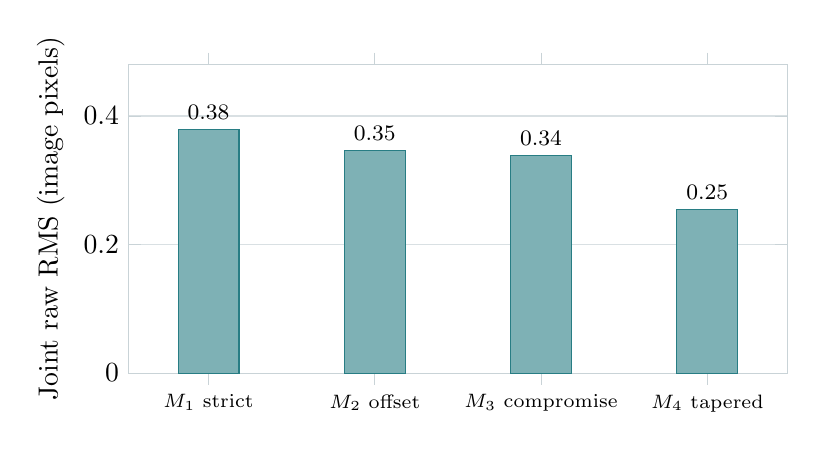
\begin{tikzpicture}
\begin{axis}[
 width=0.82\linewidth,height=5.5cm,
 ybar,bar width=22pt,
 ymin=0,ymax=0.48,
 ylabel={Joint raw RMS (image pixels)},
 symbolic x coords={Strict,Offset,Compromise,Tapered},xtick=data,
 xticklabels={\(M_1\) strict,\(M_2\) offset,\(M_3\) compromise,\(M_4\) tapered},
 x tick label style={font=\scriptsize},
 ymajorgrids=true,grid style={fine!70},
 axis line style={fine},tick style={fine},
 nodes near coords, nodes near coords style={font=\footnotesize},
 enlarge x limits=0.16]
 \addplot[fill=accent!60,draw=accent] coordinates {(Strict,0.3788) (Offset,0.3468) (Compromise,0.3389) (Tapered,0.2549)};
\end{axis}
\end{tikzpicture}
\caption{Original plot computed from the stored joint-model RMS values. The lower eight-parameter conical residual is retained as a genuine competing fit; the six-parameter strict-cylinder fit remains subpixel without independent offsets or scale changes.}
\label{fig:rms}
\end{figure}

The 6-parameter model's residuals should be understood in relation to its geometric obligations, not only relative to its competitors. It simultaneously puts the rear and near curves on one axis, fixes their common section size, and makes the measured upper exterior edge tangent to that section. Its small, distributed residuals therefore constitute positive evidence for cylindrical consistency. They do not require dismissing a more flexible competing image-plane model.

\subsection{Near- and far-termination agreement}

Independently of the joint fit, the translated unchanged near ellipse matches the far arc at \(0.18629\px\) RMS. The far curve covers only part of the termination; it has no requirement to expose its complete lower perimeter. This registration is therefore evidence that the visible part of the far terminus can carry the same local curvature as the near rim, not an observation of two complete closed end faces.

The test is stronger than a statement that each curved boundary can be approximated by an unrelated ellipse: shape, orientation, and scale are held common. It is weaker than a stereo reconstruction of both terminal planes. The distinction follows directly from the degrees of freedom and the observation geometry.

\subsection{Axis alignment and orientation identifiability}

The separate estimates for the near-ellipse minor axis, far-to-near center bearing, and upper line are \(32.704^\circ\), \(33.185^\circ\), and \(28.895^\circ\), respectively. The near ellipse is observed along an incomplete curve, allowing its angle to vary under small changes of the selected points. The reported bootstrap spread for the near-ellipse orientation is approximately \(4.23^\circ\). A transverse shift of \(1\px\) over a \(40.6\px\) center baseline changes its bearing by approximately \(1.41^\circ\). These sensitivities put the several-degree differences in context. Joint optimization chooses \(30.315^\circ\) for the strict cylinder, and achieves subpixel residuals on each point family.

\subsection{Occlusion versus intrinsic taper}

The upper exterior boundary and lower visible diagonal need not represent two opposite silhouette generators. Their measured apparent angular convergence is approximately $35^\circ$, whereas perspective convergence between parallel generators at the measured camera scale is below $0.4^\circ$ for the considered axis inclinations. This excludes the interpretation of \emph{both visible lines} as the unoccluded opposite sides of a parallel-sided body, but does not exclude a partially buried cylinder.

In the partially buried geometry, the upper transition is a material silhouette, while the lower diagonal is the contact between the body and foreground regolith. The latter can cut obliquely across a cylindrical surface as burial depth changes along its length. The two image lines therefore encode different physical boundaries, and their angular separation is not an estimator of cylinder taper without first establishing that both are true generators.

\subsection{Taper: two different statistical questions}
\label{sec:taper}

The rear-arc comparison and the coupled cone fitting answer distinct questions. A \emph{standalone} fit translates an otherwise fixed near-ellipse shape and optionally scales it by \(s\), using only 24 exposed rear points. Its minimum occurs at \(s\approx0.93\) with \(0.18434\px\) RMS, while the exact equal-size case \(s=1\) yields \(0.18629\px\), a difference of \(0.00195\px\). Across \(s=0.85\)--\(1.15\), the variations in raw residual remain small in the context of the image sampling. The conditional profile-likelihood interval recorded by the pipeline is \([0.87,0.99]\); it does not literally include \(s=1\) under that specific weighting model. Raw-fit proximity and formal confidence limits are different statements.

The \emph{coupled} eight-parameter cone fits all 85 points at once. Its best-fit \(s=0.6187\), with a nominal profile interval \([0.61,0.63]\), is associated with \(\theta\approx39.33^\circ\) and \(\alpha\approx9.46^\circ\). The taper parameter here mediates a different dependency: shrinking the far section permits the model's line of outer tangency to rotate toward the observed upper-edge angle. It obtains a lower RMS of \(0.2549\px\). That is an actual competing result, not a mismatch in the reported data.

\begin{table}[ht]
\centering\small
\caption{Two taper evaluations, with different constraints and inferential meaning. Their conditional intervals and objective functions should not be interchanged.}
\label{tab:taper}
\begin{tabularx}{\linewidth}{@{}l X X@{}}
\toprule
 & \textbf{Standalone far-arc registration} & \textbf{Coupled conical model} \\
\midrule
Observed set & 24 exposed rear points & All 85 selected points \\
Free relation & Rear center translates independently & Rear center lies on one fitted axis \\
Best diameter scale \(s\) & 0.930 & 0.619 \\
Nominal 95\% interval & [0.87, 0.99] & [0.61, 0.63] \\
Relevant residual & 0.1843 px rear RMS & 0.2549 px joint RMS \\
Equal-size comparison & 0.1863 px rear RMS at \(s=1\) & Distinct restricted joint model \(M_1\) \\
Interpretation & Partial far arc permits close equal-size registration & Taper absorbs axis/boundary angular coupling \\
\bottomrule
\end{tabularx}
\end{table}

The scientific result is not that the photograph forces a particular taper. It is that the measured boundaries admit a stringent constant-section cylindrical configuration, while an explicitly different tapered formulation also captures the image geometry. Their different axial relations matter to physical interpretation. Since the image provides one camera view of partially buried surfaces, image-plane model selection alone does not close the 3D reconstruction uniquely.

\section{Sensitivity and Repeatability}
\label{sec:sensitivity}

Measurement stability is assessed not merely by the visual appearance of fitted curves but by changing the estimation rule while keeping the scene fixed. The compiled output compares error-function transition centers, parabolically interpolated gradient maxima, and integer-pixel stations. The two subpixel methods return nearly the same upper-edge angle and consistently smaller line residuals than the discrete alternative (\cref{tab:sens}). An additional trimming experiment removes stations near the segment endpoints; the upper-line orientation shifts moderately while its central portion becomes straighter, as expected if boundary transitions are most ambiguous near neighboring objects and termini.

\begin{table}[ht]
\centering\small
\caption{Sensitivity measurements in the committed \sourcepath{measurements.json}. Values reflect alternative estimators and restricted subsets of the same target, not independent Mars images.}
\label{tab:sens}
\begin{tabularx}{\linewidth}{@{}l c c X@{}}
\toprule
\textbf{Measurement procedure} & \(\theta_{\rm upper}\) & \textbf{Upper-line RMS} & \textbf{Interpretation} \\
\midrule
Error-function subpixel & \(28.895^\circ\) & \(0.2422\px\) & Selected exterior boundary \\
Parabolic gradient peak & \(28.933^\circ\) & \(0.2105\px\) & Close independent localization rule \\
Integer-pixel positions & \(29.105^\circ\) & \(0.4559\px\) & Quantization inflates residual \\
Trim outer 15\% & \(29.154^\circ\) & \(0.1742\px\) & Central line remains straight \\
Trim outer 25\% & \(29.609^\circ\) & \(0.1195\px\) & Fewer stations and shorter baseline \\
\bottomrule
\end{tabularx}
\end{table}

In separate synthetic correlated-noise perturbations, the reported standard deviation of the apparent lower/upper convergence grows from \(1.08^\circ\) at one times empirical noise to \(2.45^\circ\) at three times noise. The method is therefore sensitive to optical sampling and pixel covariance, but the resulting uncertainty can be investigated explicitly rather than hidden behind the assumption of perfect edge localization. These tests support the stability of the selected boundaries and the value of presenting image-space residuals without converting them into unsupported manufacturing tolerances.

\section{Texture, Straightness, and Illumination as Independent Constraints}
\label{sec:comparisons}

The selected exterior edge has \(0.2422\px\) orthogonal line RMS over a sampled span of approximately \(36.4\px\). At the focus-distance reference scale that corresponds to an image-plane residual length of about \(71\,\mu\mathrm m\). This is \emph{a projected measurement residual}, not profilometric roughness of a three-dimensional surface at micrometer resolution. A quadratic curvature estimate for the same edge gives a maximum sagitta of \(0.280\px\).

Three locally selected natural rock boundaries in the same image provide a scale-matched context. Their reported line RMS values are \(0.971\), \(1.724\), and \(1.953\px\), respectively, compared with \(0.242\px\) for the target (\cref{tab:rocks}). The target edge is therefore approximately four to eight times straighter in this specific local comparison. This demonstrates anomalous local image morphology; the three contextual rocks are not an exhaustive statistical representation of all Martian geological structures.

\begin{table}[ht]
\centering\small
\caption{Same-image comparative morphology from the current report. Texture is variance of a discrete image Laplacian on normalized radiance patches.}
\label{tab:rocks}
\begin{tabularx}{\linewidth}{@{}l c c c@{}}
\toprule
\textbf{Sample} & \textbf{Edge RMS (px)} & \textbf{Relative edge RMS} & \textbf{Texture variance} \\
\midrule
Target & \textbf{0.242} & 1.0 & \(8.02\times10^{-5}\) \\
Nearby clast 1 & 0.971 & 4.0 & \(1.64\times10^{-4}\) \\
Nearby clast 2 & 1.724 & 7.1 & \(2.45\times10^{-4}\) \\
Nearby clast 3 & 1.953 & 8.1 & \(2.98\times10^{-4}\) \\
\bottomrule
\end{tabularx}
\end{table}

An additional radiometric test examines intensity across the upper body, fitting a transverse profile \(I(v)=c_0+c_1v+c_2v^2\). The selected-profile comparison in the repository gives a curvature significance as high as \(z=11.45\) for selected sections relative to a planar-gradient null hypothesis \(c_2=0\). The broader modeling record also includes alternative profile selections and illumination treatments. These shading results support a smoothly convex illuminated surface but are not themselves unique to a cylinder; mineral albedo, local scattering, dust, and illumination geometry can alter brightness profiles.

The smoothness, curved terminal boundaries, and tangency-constrained joint fit are complementary constraints. None should be substituted for the others, and the most informative result is their common geometric compatibility.

\section{Geological and Manufactured-Origin Interpretations}
\label{sec:origin}

\subsection{What a physical explanation must account for}

The image supports three separate types of statement. \emph{Observation}: there are identifiable near and far curved terminations, a high-contrast outer longitudinal edge, and a soil/shadow boundary with different geometry. \emph{Model}: a common constant-section cylinder fits the selected geometric points to a subpixel residual. \emph{Origin}: a claim that the object formed naturally, was manufactured, or arrived through some transport process. The first two constrain the third but do not automatically determine it.

A viable origin hypothesis must explain the observed curvature and location of both ends, the longitudinal straightness and surface texture, the apparent burial, and the solar-shadow relationship. A named process is a category of candidate mechanisms, not a numerical reconstruction of this particular object.

\subsection{Wind abrasion and sedimentary fracture}

Ventifacts are genuinely common in Gale crater, with documented facets, keels, flutes, grooves, and wind-related abrasion textures \cite{bridges2014}. The local lithology in the repository is characterized as layered sandstones and sulfate-bearing fine sediments, offering plausible sources of spalls, slabs, and weathered fragments. Erosion and fracture can generate smooth arcs and nearly straight edges over small distances, and a burial margin can make a roughly wedge-like rock resemble a more symmetric solid.

The particular challenge for a simple wind-shaped clast explanation is quantitative: it must reproduce the close near/far translated curvature and the narrow six-parameter joint fit while respecting the physical distinction between material silhouette and regolith contact. The local natural-clast comparisons in \cref{tab:rocks} do not provide such a matching mechanism. They therefore strengthen the case that this target is morphologically unusual within its immediate scene, without establishing a universal exclusion theorem for natural rock formation.

\subsection{Pipe concretions and fluidized-sediment structures}

Natural cylindrical structures are geologically real. Iron-oxide pipelike concretions in the Navajo Sandstone can develop around self-organized cylindrical reaction fronts \cite{loope2011}. Gale crater also contains structures interpreted as fluidized-sediment pipes, some with concentric or eccentric layering \cite{rubin2017}. These are more relevant comparator mechanisms than a generic assertion that wind ``makes round rocks.''

However, demonstrating that a geological process produces pipes is not the same as demonstrating that it produces \emph{this specific small, apparently separated body}, with its selected pair of terminating curves, exterior straightness, and buried context. The existing repository compares expected rind structure, grain-scale texture, irregularity, and terminal fracture morphologies. No quantitatively specified natural mechanism in the present record has yet reproduced the entire 85-point observation set. The repository's structural result therefore remains an anomaly requiring a case-specific process explanation, rather than being resolved by an analogy alone.

\subsection{Manufactured-object and rover-hardware hypotheses}

Constant-section pins, sleeves, tubes, bushings, and related engineered elements naturally possess the exact class of geometry tested by \(M_1\). This makes manufacture a morphologically motivated hypothesis, not merely an inference from resemblance. A separate hardware and transport assessment in the repository compares candidate mission components, landing-site separation, rover traverses, and possible transport pathways. It does not identify a documented Curiosity component matching this image as a confirmed local source.

The measured geometry cannot identify metal versus stone, hollow tube versus solid rod, or terrestrial hardware versus any other manufacturing history. The image also does not provide material spectroscopy on the object. Manufacturing origin is therefore an interpretive hypothesis supported by morphological correspondence, not a compositional measurement. The narrow result of the present study is the object's unusually precise compatibility with a cylindrical model.

\section{Integrated Evaluation and Scope}
\label{sec:discussion}

The case for cylindrical geometry is cumulative. The near rim is an accurately sampled smooth curve. A separate far arc accepts an unchanged translated version of that near curve. The measured upper exterior line is exceptionally straight and lies at the offset expected for the near rim's radius. Their shared six-parameter model fits 85 points without an independent rear scale, an adjustable upper crest, or independently wandering centers. The observation cannot be reduced to one elliptical fit or one visually suggestive edge.

The shared model is consequential because each observed feature constrains a different part of its geometry. Near and far terminal curvature determine the projected section; their relative positions constrain the common axis; and the exterior line imposes tangency at the same transverse radius. These requirements are solved simultaneously, rather than assembled as a sequence of individually plausible visual matches.

The comparison with a tapered frustum provides a different kind of information. Its lower residual is genuine within the chosen image-plane model, and its tight conditional scale-ratio interval follows from the coupling imposed on its axis and silhouette. That model should not be collapsed into the separate far-arc scale experiment, whose nearly unchanged residual at \(s=1\) is also genuine. The two fits encode different hypotheses about the mapping between observed boundaries and physical surfaces.

The most defensible classification is consequently \textbf{a strongly supported cylindrical image-plane morphology for a partially buried object}. This directly constrains any proposed origin. The claim is neither a mere visual impression nor a material assay. To distinguish the strict cylinder from physically different 3D configurations, one additional viewing azimuth, a target-centered stereo pair, or a resolved surface/topography measurement would be decisive. The reported pixel-level measurements already stand independently as a quantitative research result.

\section{Reproducibility and Data Availability}
\label{sec:reproduce}

The complete source archive and machine-readable numerical outputs are available in \repo. The numerical snapshot used for this manuscript is the default-branch commit
\begin{quote}\small\ttfamily\color{ink}
90fbf8f89ac2634a9dbd2b27f81fc80d68b9943c
\end{quote}
The scientific scripts reside in \sourcepath{independent-reconstruction/}. The recorded processing order begins with \sourcepath{step1_image_inspection.py} (provenance), proceeds through camera modeling, feature extraction, conic comparison, interpretations, near/far terminal analysis, and joint modeling, and ends with robustness compilation. The module \sourcepath{run_all.py} orchestrates that workflow.

\begin{lstlisting}[language=bash,caption={Re-execution from a local repository checkout containing the PDS image data.}]
python -m pip install -r independent-reconstruction/requirements.txt
python independent-reconstruction/run_all.py
\end{lstlisting}

Primary output files are \sourcepath{step3_features.json} for measured stations and their uncertainty/contrast metadata; \sourcepath{step4_endface_models.json} for candidate end-curve fits; \sourcepath{step8_pebble_and_rear_terminus.json} for the physical near/far segmentation; \sourcepath{step9_joint_model.json} for shared-axis models and both taper profiles; and \sourcepath{measurements.json} for compiled camera and sensitivity metrics. All values in this paper are traceable to that committed record. The figure in this manuscript is an original vector visualization constructed from the reported numerical values, not a reproduced repository figure.

The reproducibility standard for extending the study is straightforward: retain pixel coordinates and provenance, document each boundary as a material or shadow transition, state model parameters and constraints, and report both raw pixel residuals and the assumed measurement-uncertainty model. The geometrical explanation can then be challenged or improved without substituting narrative plausibility for the observed data.

\section{Conclusion}

Physically directed subpixel measurements of the sol-3556 Mastcam-100 image yield three mutually constraining geometric features: a 35-point near curved rim, a 24-point exposed far termination, and a 26-point straight upper exterior boundary. The near arc is fit by an ellipse at \(0.164\px\) RMS; an equal-size translated copy registers to the exposed far arc at \(0.186\px\). Their strict common-axis, common-section, tangent-boundary representation fits all 85 observations at \(0.3788\px\) RMS with six parameters. This is quantitative and reproducible evidence of cylindrical morphology on Mars, not simply an assessment of visual similarity.

The analysis distinguishes progressive burial from physical taper, identifies cast shadow as a separate image boundary, and includes a more flexible eight-parameter tapered fit as a competing projection. Local smoothness measurements show the target's upper boundary to be substantially straighter than three neighboring rock edges. These results place a concrete geometric burden on explanations based on sandstone fracture, wind abrasion, diagenetic pipe formation, or manufactured hardware.

The present image establishes the geometry to the resolution and assumptions of the available measurements. It leaves material identity, object origin, and unique three-dimensional structure for evidence capable of deciding those separate questions.

\section*{Acknowledgment and provenance note}
\addcontentsline{toc}{section}{Acknowledgment and provenance note}
The calculations and data products synthesized here were developed in the public \emph{martian-cylinder} research repository, using NASA Mars Science Laboratory data. Repository provenance is attributed explicitly; this paper is a synthesis of the recorded investigation, not a claim of independently reacquiring a second rover observation. No NASA institutional endorsement is implied.

\begin{thebibliography}{99}\setlength{\itemsep}{4pt}
\bibitem{bogner2026repo} Bogner, J. (2026). \emph{Martian-cylinder: Independent reconstruction of Curiosity Sol 3556 Mastcam-100 imagery}. Cambrian Minds Media, source code, technical reports, image products, and numerical output. \url{https://github.com/CambrianMinds/martian-cylinder/tree/90fbf8f89ac2634a9dbd2b27f81fc80d68b9943c}.
\bibitem{pds} NASA Planetary Data System and Malin Space Science Systems. \emph{Mars Science Laboratory Mastcam RDR image product \pdsid}; dataset \texttt{MSL-M-MASTCAM-4-RDR-IMG-V1.0}, sol 3556, 7 August 2022. PDS3 labels and image arrays distributed with the repository snapshot.
\bibitem{malin2017} Malin, M. C., et al. (2017). The Mars Science Laboratory (MSL) Mast cameras and Descent Imager: Investigation and instrument descriptions. \emph{Earth and Space Science}, 4, 506--539. \url{https://doi.org/10.1002/2016EA000252}.
\bibitem{bell2017} Bell, J. F., III, et al. (2017). The Mars Science Laboratory Curiosity rover Mastcam instruments: Preflight and in-flight calibration, validation, and data archiving. \emph{Earth and Space Science}. \url{https://doi.org/10.1002/2016EA000219}.
\bibitem{bridges2014} Bridges, N. T., et al. (2014). The rock abrasion record at Gale Crater: Mars Science Laboratory results from Bradbury Landing to Rocknest. \emph{Journal of Geophysical Research: Planets}, 119, 1374--1389. \url{https://doi.org/10.1002/2013JE004579}.
\bibitem{loope2011} Loope, D. B., Kettler, R. M., and Weber, K. A. (2011). Morphologic clues to the origins of iron oxide-cemented spheroids, boxworks, and pipelike concretions, Navajo Sandstone of south-central Utah, U.S.A. \emph{The Journal of Geology}, 119, 505--520. \url{https://doi.org/10.1086/661110}.
\bibitem{rubin2017} Rubin, D. M., et al. (2017). Fluidized-sediment pipes in Gale crater, Mars, and possible Earth analogs. \emph{Geology}, 45(1), 7--10. \url{https://doi.org/10.1130/G38339.1}.
\bibitem{chan2004} Chan, M. A., Beitler, B., Parry, W. T., Orm\"o, J., and Komatsu, G. (2004). A possible terrestrial analogue for haematite concretions on Mars. \emph{Nature}, 429, 731--734. \url{https://doi.org/10.1038/nature02600}.
\end{thebibliography}

\appendix
\section{Detailed Measurement Inventory}
\label{app:inventory}

\begin{table}[ht]
\centering\small
\caption{Feature-level source coordinates and elementary fits. All coordinates refer to zero-based DRXX pixels.}
\begin{tabularx}{\linewidth}{@{}l l l X@{}}
\toprule
\textbf{Feature} & \textbf{Count} & \textbf{Observed region} & \textbf{Output / relation} \\
\midrule
Near rim & 35 & \(x:1051.52\)--\(1083.73\); \(y:967.15\)--\(994.17\) & Unconstrained ellipse \(a=19.717\), \(b=16.424\), \(0.164\px\) RMS \\
Far cap & 24 & \(x:1027.91\)--\(1039.23\); \(y:945.40\)--\(949.86\) & Equal-size translated near ellipse, \(0.186\px\) RMS \\
Upper edge & 26 & \(x:1036.84\)--\(1069.03\); \(y:945.40\)--\(962.55\) & ODR line \(28.895^\circ\); \(0.242\px\) RMS \\
Shared fit & 85 & Combined regions & Strict cylinder: \(30.315^\circ\), \(0.379\px\) RMS \\
\bottomrule
\end{tabularx}
\end{table}

The near-rim set retains 35 of 36 sampled radial stations after excluding the station at \(-45^\circ\) that crosses onto the adjacent pebble. The far arc is the bounded exposed portion of a 36-point extraction, excluding both the burial contact and the transition to the upper longitudinal boundary. These criteria are feature-based rather than chosen only by minimizing a fitted residual.

\section{Projection and Identifiability Details}
\label{app:projection}

For an ideal projected circular end plane with normal aligned to the three-dimensional cylinder axis, the end appears elliptical under oblique viewing. In an orthographic approximation its axis ratio satisfies \(b/a\approx|\cos\gamma|\), where \(\gamma\) is the angle between the end-plane normal and the line of sight. The repository's unconstrained near-ellipse ratio \(b/a=0.833\) is therefore compatible with \(\gamma\approx33.6^\circ\), subject to perspective and local projection convention. Its orientation is much less stable than its point-to-ellipse residual because only a partial arc is observed.

The projected position of an unobserved ellipse center is similarly uncertain. Over a short terminal arc, changes in scale and center position can compensate, allowing a one-to-one translation to reproduce the observed curve with only small increases in RMS. This is why rear curvature should be reported as a constraint on the \emph{visible arc}, rather than a direct measurement of the entire concealed end plane. When coupled to a longitudinal surface hypothesis, the same feature gains additional predictive meaning: its center and scale can no longer change independently.

For the strict model, local coordinates of a measured upper-edge point \(\mat x_d=(x_d,y_d)\) are
\begin{align}
 u_d&=(x_d-x_f)\cos\theta+(y_d-y_f)\sin\theta,\\
 v_d&=-(x_d-x_f)\sin\theta+(y_d-y_f)\cos\theta.
\end{align}
The tangent residual \(e_d=v_d+a\) follows immediately from \cref{eq:tangent}. Its sign and the image coordinate orientation are not cosmetic: reversing the orientation of the extracted intensity boundary changes which physical contour is being compared with this equation.

\section{Sensitivity, Resolution, and Error Interpretation}
\label{app:error}

The spatial residual \(0.3788\px\) is not the per-point localization uncertainty, the actual physical surface error of the object, or the probability that a cylinder is true. It is the raw root-mean-square distance of selected image observations from one defined six-parameter model. At the reference image scale from \cref{eq:scale}, it corresponds to about \(0.111\,\mathrm{mm}\) in the projected image plane.

The workflow samples several overlapping descriptions of the same optical signal: error-function transition centers, parabolically interpolated gradient extrema, three radiance bands, linearized camera products, and trimmed subsets. Reassuring agreement across these comparisons demonstrates stability to those processing choices. Because neighboring stations and demosaiced bands are not fully independent, the effective number of independent observations for formal significance testing may be less than the literal station count. The six-parameter fit remains a reproducible geometric description regardless of how a future error covariance model is refined.

Physical measurements in millimeters depend linearly on assumed distance \(D\). For the strict cylinder, the transverse diameter \(2a\approx39.99\px\) scales to approximately \(10.70\)--\(13.07\,\mathrm{mm}\) across the nominal focus-search interval \(3.6\)--\(4.4\,\mathrm m\), or \(11.76\,\mathrm{mm}\) at \(3.957\,\mathrm m\). The projected center separation \(40.86\px\) is \(12.0\,\mathrm{mm}\) at that same assumed distance; the full three-dimensional object length is not the same quantity and requires orientation reconstruction. Distinguishing projected separation from body length prevents the focus-distance scenario from being mistaken for direct ranging.

\section{File Integrity and Analysis Snapshot}
\label{app:hash}

The provenance manifest records the following SHA-256 digests for primary images. These allow future readers to verify that the same byte-level image arrays are being analyzed.

\noindent{\scriptsize\ttfamily
\begin{tabularx}{\linewidth}{@{}l X@{}}
\toprule
DRXX & 45a3d5e5d32ed823e8a3e2ff0dc0f5ffeb5bd546c81be8d51e06c9f241b5e1fd \\
DRLX & 911e661c99a4453f4b3d4bd13a3d35f049c5df965fcb3c91b014a47c38c7605f \\
DRCX & 8aec700e07d61123151c0811332f76e10f13d1e3fb361de5b10476b4961c473f \\
DRCL & 761c9c1774cfe5152ca7d5cb729de285d08fa78c3df05af8720cbd9599b37592 \\
\bottomrule
\end{tabularx}
}

\medskip
\noindent The paper's cited commit freezes the interpretation and the accompanying JSON values used here. Updated repository commits should be treated as new versions of the research record, not silently substituted for this snapshot in reproducing numerical tables.

\end{document}
